\documentclass[border=10pt]{standalone}

\usepackage{tikz}
\usepackage{tikzsymbols}
\usetikzlibrary{calc,patterns,shapes.geometric}

\def\centerarc[#1](#2)(#3:#4:#5){\draw[#1] ($(#2)+({#5*cos(#3)},{#5*sin(#3)})$) arc (#3:#4:#5);}

\begin{document}
	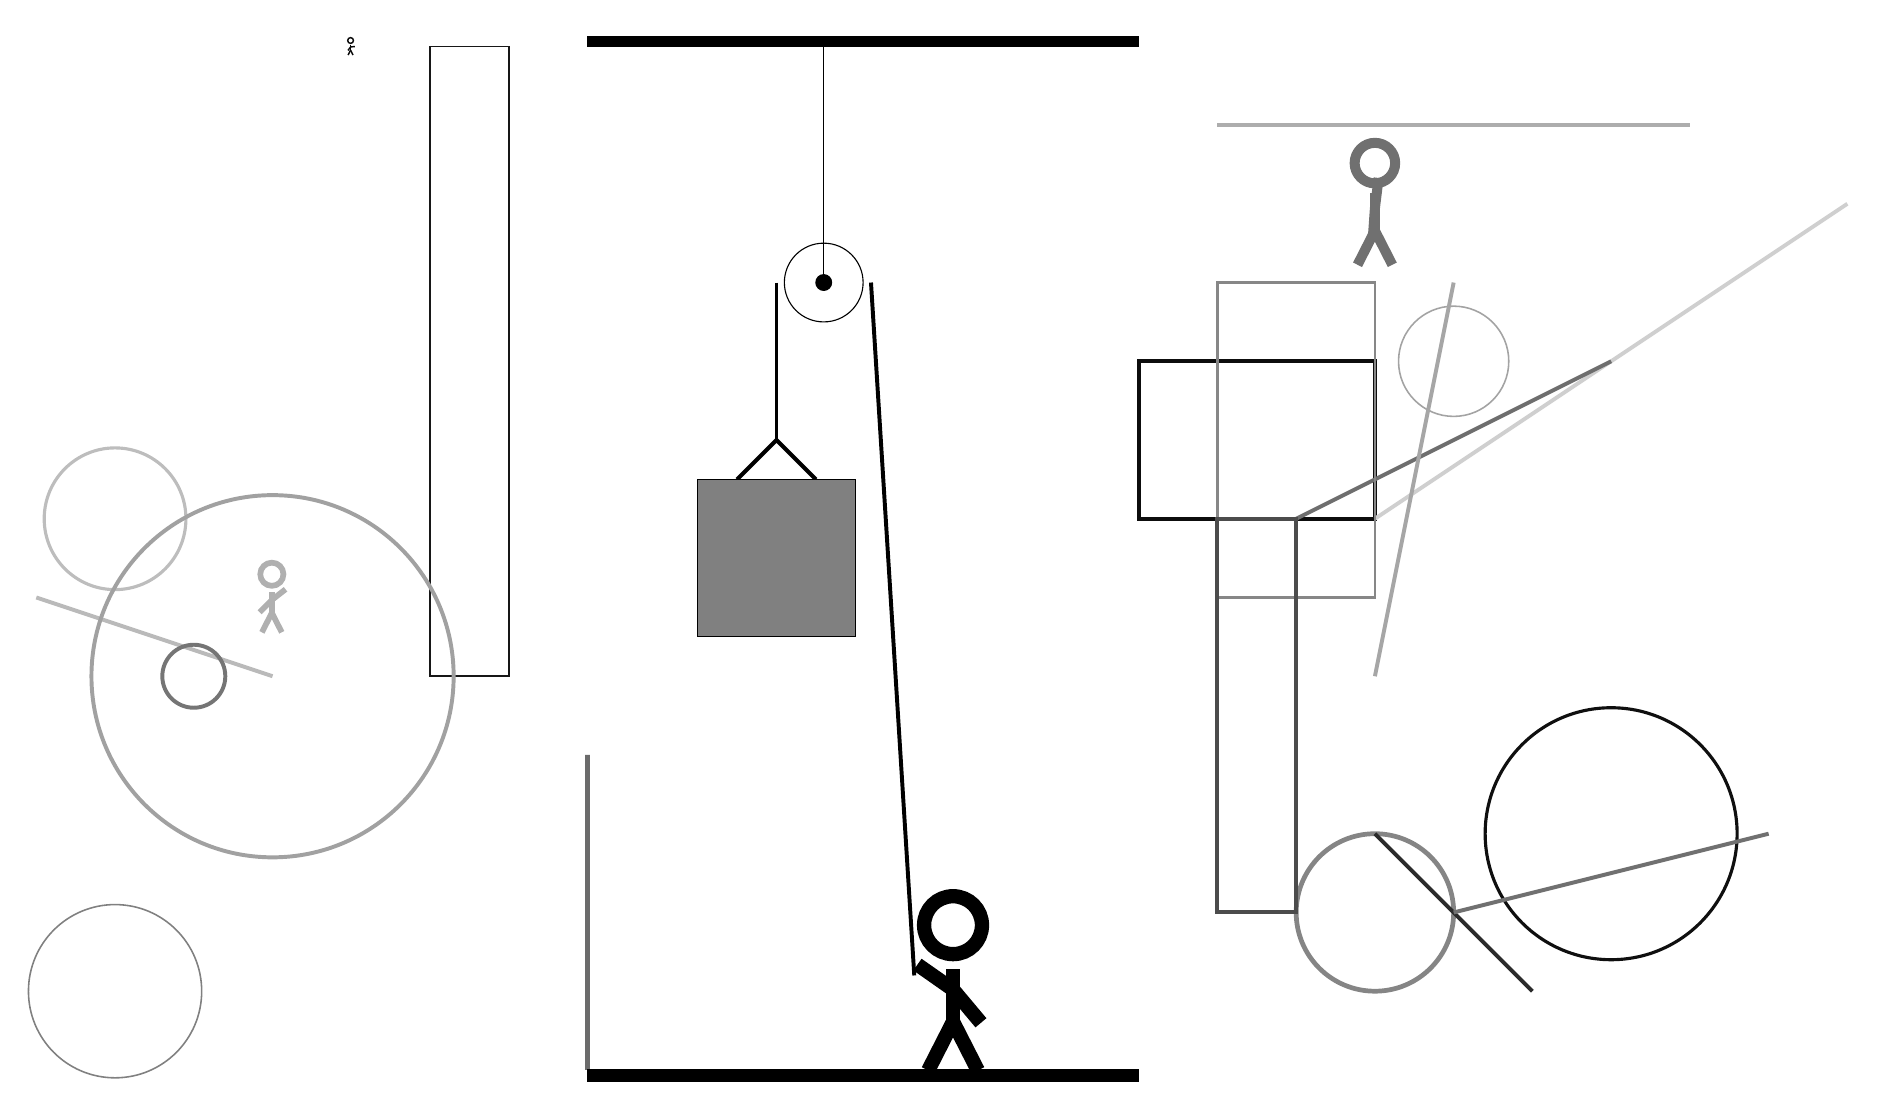
\begin{tikzpicture}
		%%%%% START %%%%%
		
		\draw[fill=black] (-2, 10) rectangle (5, 10.125);
		
		\draw (1, 7) circle (0.5);
		\draw[fill=black] (1, 7) circle (0.1);
		\draw (1, 10) -- (1, 7);
		
		\draw[line width=0.5mm] (-0.1, 4.5) -- (0.4, 5.0) -- (0.9, 4.5);
		\draw[fill=black!50] (-0.6, 4.5) rectangle (1.4, 2.5);
		
		\draw[line width=0.5mm] (0.4, 7) -- (0.4, 5.0);
		\centerarc[line width=0.5mm](1, 7)(0:180:0.6);
		\draw[line width=0.5mm](1.6, 7) -- (2.15, -1.8);
		
		\node at (2.6, -1.9) {\Strichmaxerl[10][-35][-50]};
		
		\draw[line width=0.2mm, color=black!91] (-4, 2) rectangle (-3, 10);
		
		\node[line width=0.6mm, color=black!31] at (-6, 3) {\Strichmaxerl[4][45][38]};
		\draw[line width=0.5mm, color=black!95] (5, 4) rectangle (8, 6);
		\draw [line width=0.4mm, color=black!94](11, 0) circle (1.6);
		
		\draw [line width=0.6mm, color=black!48](8, -1) circle (1.0);
		
		\draw[line width=0.5mm, color=black!27](-6, 2) -- (-9, 3);
		\draw[line width=0.5mm, color=black!19](8, 4) -- (14, 8);
		
		\draw [line width=0.2mm, color=black!50](-8, -2) circle (1.1);
		\draw[line width=0.5mm, color=black!83](8, 0) -- (10, -2);
		\draw[line width=0.5mm, color=black!32](6, 9) -- (12, 9);
		\draw [line width=0.4mm, color=black!26](-8, 4) circle (0.9);
		
		\draw[line width=0.5mm, color=black!57](7, 4) -- (11, 6);
		\draw[line width=0.3mm, color=black!47] (6, 7) rectangle (8, 3);
		
		\draw [line width=0.2mm, color=black!36](9, 6) circle (0.7);
		\node[line width=0.2mm, color=black!96] at (-5, 10) {\Strichmaxerl[1][53][5]};
		\draw[line width=0.7mm, color=black!58] (-2, -3) rectangle (-2, 1);
		
		\draw[line width=0.5mm, color=black!35](8, 2) -- (9, 7);
		\draw [line width=0.5mm, color=black!37](-6, 2) circle (2.3);
		\draw [line width=0.5mm, color=black!54](-7, 2) circle (0.4);
		\draw[line width=0.5mm, color=black!56](9, -1) -- (13, 0);
		\node[line width=0.7mm, color=black!56] at (8, 8) {\Strichmaxerl[7][86][83]};
		
		\draw[line width=0.5mm, color=black!70] (7, 4) rectangle (6, -1);
		
		
		\draw[fill=black] (-2, -3) rectangle (5, -3.15);
		
		%%%%% END %%%%%
	\end{tikzpicture}
\end{document}